\section{Bayesian Neural Networks}

In the previous section, we explored into one of the most popular classes of ML algorithms, ANNs, and discussed some of the challenges and limitations they face. In this section, it will be introduced an alternative approach that can mitigate these issues.

\subsection{Bayesian approach}

One way to address the overconfidence problem is by employing the \textit{Bayesian} theory, which offers a rigorous framework to enhance learning in ML. Bayesian theory provides a general approach to probability, encompassing the \textit{frequentist} approach as a special case, even though they are often viewed as contrasting approaches \cite{noauthororeditor}. 

The frequentist approach relies on the concept of repeated sampling, where probabilities are defined by their connection to countable events and their frequencies in very large samples. Within this framework, parameters are considered fixed and unknown, and the primary objective is to accurately estimate them or test hypotheses based on observed data. Therefore, parameters cannot have probability distributions, only the data sampled can.

In contrast, the Bayesian framework combines prior knowledge or beliefs about a parameter with observed data to form a posterior distribution, which reflects updated beliefs about the parameter after considering the data. Bayesians treat parameters as random variables and use probability distributions to model them. This facilitates the integration of uncertainty estimation into the analysis. Bayesian inference is based on the Bayes' theorem, which is expressed as follows:

\begin{equation} \label{eq:1}
	P(A|B) = \frac{P(B|A) \cdot P(A)}{P(B)}
\end{equation}

In \Eq~\ref{eq:1} $P(B)$ represents the prior knowledge while $P(B|A)$ is the likelihood of observing B given A. Within ML applications $A$ typically represents the model parameters, while $B$ the observed data. The prior knowledge $P(B)$ encapsulates any existing information or beliefs about the data before observing the actual evidence. It serves as initial estimation of the likelihood. The posterior distribution, denoted as $P(A|B)$, represents the updated beliefs about the model parameters $A$ after considering the evidence from the data.

The differences and main aspects of the two approaches mentioned above are outlined in \Tab~\ref{table:BayesVsFreq}.

\begin{table}[h]
	\centering
	\begin{tabular}{|| l | l | l ||} 
		\hline
		\textbf{Aspect} & \textbf{Bayesian} & \textbf{Frequentist} \\
		\hline
		\hline
		Parameters & Treated as random variables. & Considered fixed but unknown. \\
		Prior knowledge & Yes. & No. \\
		Inference & Based on posterior. & Based on likelihood. \\
		Parameter estimation & A probability distribution. & A single point. \\	
		Uncertainty Estimation & Inherently incorporated. & Often not explicitly addressed. \\	
		\hline
	\end{tabular}	
	\caption{Comparison of Bayesian and frequentist Approaches}
	\label{table:BayesVsFreq}
\end{table}

\subsection{Bayesian approach to neural networks}

As mentioned at the outset of this section, ANNs face certain limitations that can be effectively addressed through the utilization of Bayesian inference. 
This has led to the development of Bayesian neural networks (BNNs), which are commonly defined as \textit{stochastic} ANNs trained using Bayesian inference. Unlike conventional ANNs with fixed single weights, BNNs specify a distribution over the weight parameters. 
Consequently, during training, Bayesian inference techniques are employed, allowing BNNs to leverage the combined advantages of ANNs and principles of probabilistic modeling. In \Fig~\ref{fig:annvsbnn} it is shown graphically the main difference between ANN and BNN.

A graphical representation of the main difference between ANN and BNN is illustrated in \Fig~\ref{fig:annvsbnn}.

\begin{figure}[h]
	\centering
	\begin{subfigure}{.5\textwidth}
		\centering
		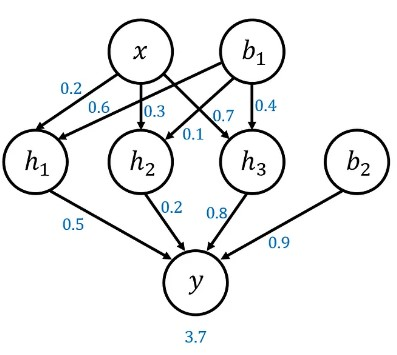
\includegraphics[width=0.8\linewidth]{ImageFiles/BayesianNeuralNetworks/ANN}
		\caption{Example of an ANN}
		\label{fig:ann}
	\end{subfigure}%
	\begin{subfigure}{.5\textwidth}
		\centering
		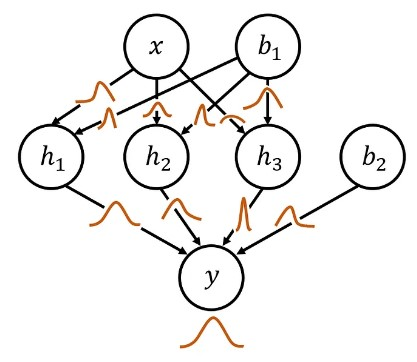
\includegraphics[width=0.8\linewidth]{ImageFiles/BayesianNeuralNetworks/BNN}
		\caption{Example of a BNN}
		\label{fig:bnn}
	\end{subfigure}
	\caption{ANN vs BNN \cite{WYSUBNN}}
	\label{fig:annvsbnn}
\end{figure}

BNNs can be interpreted as a set of infinite networks rather than a single fixed model. This is due to the fact that BNNs represent weight parameters as probability distributions. Each model is then defined by a different draw from the posterior distribution over weights. This unique characteristic of makes them particularly well-suited for uncertainty quantification and robustness analysis. 

\subsection{Inference algorithms}

As previously mentioned, the training process employs Bayesian inference. In other words, it aims to calculate the posterior by utilizing a prior distribution. However, this task can be challenging due to the potential complexity of the integrals involved, making them intractable in many cases. Consequently, specialized algorithms are required to tackle this issue. The two most widely used approaches are Markov chain Monte Carlo (MCMC), which is a sampling technique, and \textit{variational} inference, which seeks to approximate the posterior.

\vspace{0.2cm}
\textbf{Markov chain Monte Carlo}

Markov chain Monte Carlo (MCMC) is a powerful class of computational algorithms used for sampling from complex probability distributions. It is particularly useful when direct sampling from the target distribution is impractical or impossible. By generating a sufficiently large sample size, important statistics like mean and variance can be computed.

At the core of MCMC lies the concept of Markov chains, which are stochastic processes satisfying the Markov property, i.e., the future state of the process relies only on its current state, independent of its past states. 
In the context of MCMC, the idea is to create a Markov chain, i.e., a sequence of random samples denoted as $S_i$—where each sample $S_i$ is probabilistically dependent only on the preceding sample $S_{i-1}$. 
This construction is done such that the $S_i$ samples are distributed according to the desired distribution. However, it's important to note that not all the samples $S_i$ are stored, as they may exhibit autocorrelation. In practice, most MCMC algorithms require an initial burn-in time to allow the Markov chain to converge towards the desired distribution.
In \Fig~\ref{fig:mcmc}, a graphical representation illustrates the macro operations involved in the family of MCMC algorithms.

\begin{figure}[h]
	\centering
	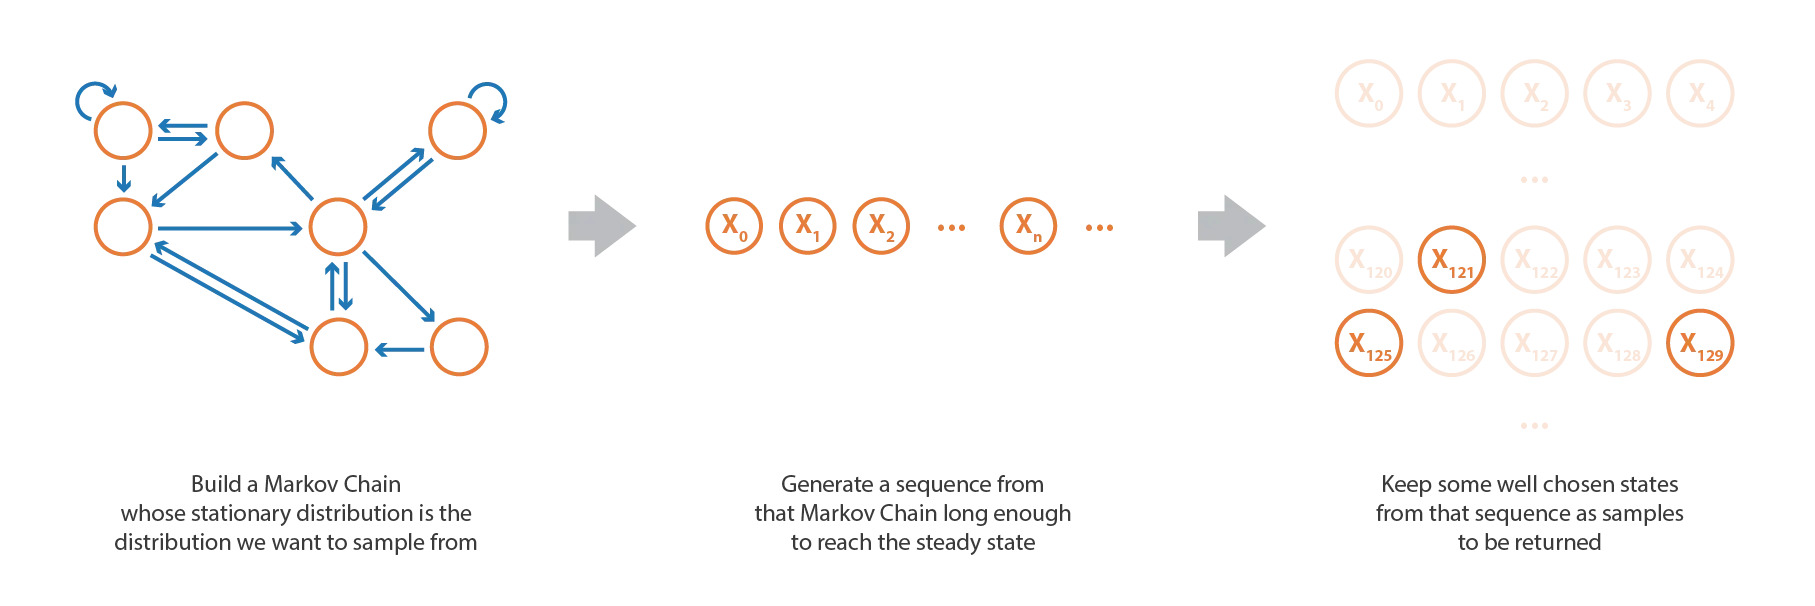
\includegraphics[width=0.8\linewidth]{ImageFiles/BayesianNeuralNetworks/mcmc}
	\caption{Functioning of the MCMC algorithms \cite{BIPMCMCV}}
	\label{fig:mcmc}
\end{figure}

Regarding Bayesian deep learning, not all MCMC methods are relevant. The most popular and widely used within the context of BNNs is the \textit{Metropolis-Hastings} algorithm.

Indeed, while MCMC algorithms are powerful for sampling from exact posterior distributions, they do face limitations in terms of scalability. As the size of the model grows, applying MCMC becomes increasingly computationally expensive and, in some cases, infeasible.

\vspace{0.2cm}
\textbf{Variational inference}

This family of techniques aims to find the optimal approximation of the desired distribution. This approach involves a distribution, denoted as $q_{\phi}(H)$, which is referred to as the variational distribution, parameterized by a set of parameters $\phi$. The goal is to learn the values of $\phi$ such that the distribution $q_{\phi}(H)$ approximates the exact posterior. In essence, the inference problem is transformed into an optimization problem, where the objective is to minimize the discrepancy between the variational distribution and the true posterior distribution. The idea behind this approach is illustrated in \Fig~\ref{fig:vi}. By iteratively refining the parameters $\phi$, the variational distribution becomes a better approximation of the exact posterior. This optimization process allows variational inference to be more scalable and computationally efficient than traditional MCMC methods, especially in scenarios where direct sampling from the posterior is not feasible.

\begin{figure}[h]
	\centering
	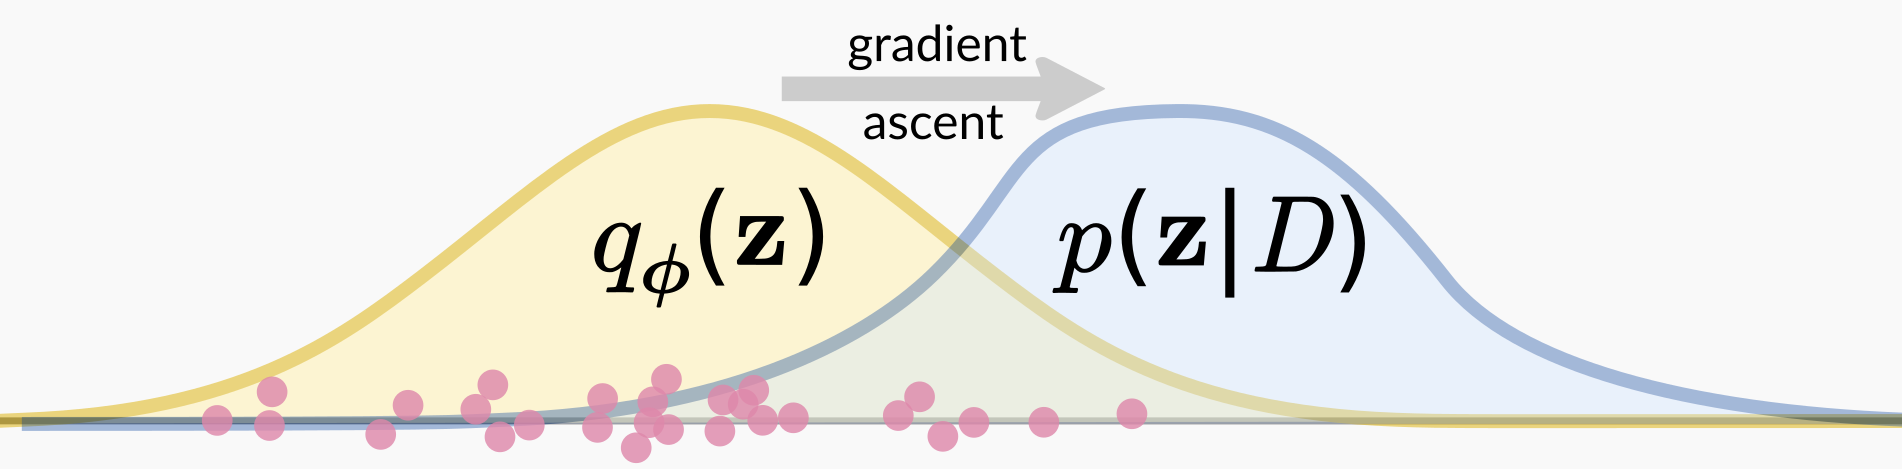
\includegraphics[width=0.8\linewidth]{ImageFiles/BayesianNeuralNetworks/vi}
	\caption{Variational inference \cite{VBPI}}
	\label{fig:vi}
\end{figure}

To measure discrepancy  between the two probability distributions, the Kullback-Leibler divergence (KL-divergence) is commonly used.  It is a concept from information theory, specifically based on Shannon's information theory, and it provides a measure of how one distribution diverges from another.

\[
	D_{KL}(q_{\phi} || P) = \int_{H} \ q_{\phi}(H') \ log(\frac{q_{\phi}(H')}{P(H'|D)}) dH'
\]

Using this formula, it becomes possible to quantify the difference between two probability distributions. In fact, when the variational distribution $q$ is equal to the true posterior $P$ (i.e., $q = P$), the KL-divergence $D_{KL}(q_{\phi} | P)$ becomes zero.

However, it is not possible to compute the exact formula since $P(H|D)$ is not known. To overcome this problem, the idea is to use unnormalized probability distribution $\hat{P}$.
From \Eq~\ref{eq:1}, it follows that $\hat{P} = P(H|D)P(D) = P(D|H)P(H)$. Using the definition of conditional probabilities, $P(D|H) = \frac{P(D,H)}{P(H)}$, which implies that $\hat{P} = P(D,H)$. 

The objective function becomes:

\[
	\int_{H} \ q_{\phi}(H') \ log(\frac{q_{\phi}(H')}{P(H',D)}) dH' = D_{KL}(q_{\phi} || P) - log(P(D))
\]

This quantity is referred to as the \textit{evidence lower bound} (ELBO). Since $log(P(D))$ depends only the prior, minimizing $D_{KL}(q_{\phi} || P)$ is equivalent to minimizing the ELBO.

A crucial consideration at this stage is the selection of the family of distributions, denoted as $Q$. This choice is important for controlling both the bias and the convergence rate of the variational inference process \cite{doi:10.1080/01621459.2017.1285773}. Here arises a trade-off between convergence velocity and bias. Opting for a more complex family of distributions would result in increased computational complexity but lower bias. Conversely, opting for a simpler family would lead to faster convergence but a higher bias.

A common choice employed in ML is the \textit{mean-field variational} family \cite{Han2019StatisticalII}. This type of variational inference relies on making an independence assumption over the variables. Consequently, the variational distribution can be expressed as follows:
\[
	q(x) = \prod_{j=1}^{m} q(x_j)
\] 
where $m$ is the dimension of the distribution. Each component $q(x_j)$ corresponds to a one-dimensional probability distribution. This factorization assumption simplifies the optimization problem and allows for more efficient computation during the variational inference process.

\vspace{0.2cm}
\textbf{Comparing MCMC and  Variational inference}

MCMC methods are generally more computationally intensive compared to variational inference. However, they offer the advantage of producing (asymptotically) precise samples from the target density. On the other hand, variational inference is faster but operates as an approximation method without any assurance of exact convergence.

Therefore, MCMC is better suited for smaller data sets and situations where the computational cost can be justified to obtain more accurate samples. In contrast, variational inference is ideal for handling large data sets and scenarios where the priority lies in the exploration of numerous models.

\subsection{Uncertainty estimation}

As presented at the beginning of this section, one of the key advantages of BNNs is the uncertainty estimation. This is very important in critical safe applications to make robust decisions based on the confidence of the predictions. BNNs allow to quantify inherently the uncertainty. Furthermore, they allow the decomposition of the predictive uncertainty into two parts: aleatoric and epistemic uncertainty \cite{Mitros2019OnTV}.

\vspace{0.2cm}
\textbf{Aleatoric uncertainty}

Aleatoric uncertainty, also known as data uncertainty, refers to the inherent stochasticity present in the process being modeled with a BNN (Bayesian Neural Network). This kind of uncertainty emerges from noisy and ambiguous data points. It represents an error that cannot be eliminated even with the addition of more data \cite{article01}. This type of uncertainty can be interpreted as the network's knowledge about a specific input. When a data point is very different from the ones used during training, the network would provide a prediction with a higher uncertainty.

\vspace{0.2cm}
\textbf{Epistemic uncertainty}

Epistemic uncertainty, also referred to as model uncertainty, represents the uncertainty on the model parameters. Within the context of BNNs, epistemic uncertainty captures the uncertainty in the model structure and architecture. This type of uncertainty can be reduced by acquiring more data or by employing a different model architecture. It can also be used as a metric for assessing the model quality.

\vspace{0.2cm}
\textbf{Combining Epistemic and Aleatoric Uncertainty}

BNNs offer the capability to simultaneously incorporate both aleatoric and epistemic uncertainties. Through this combination, a more comprehensive and precise estimation of the overall uncertainty in predictions can be achieved. To achieve this, one can simply sum the two quantities. However, in this work, the focus will be placed on the aleatoric uncertainty rather than the epistemic uncertainty.